\section{Evolúciós játékok}

\subsection{Klasszikus játékelméleti fogalmak}
\begin{frame}
\frametitle{Klasszikus játékelméleti fogalmak}
\begin{itemize}
	\item játék, játékosok
	\item a cél a nyereség maximalizálása
	\item Nash-egyensúly
\end{itemize}
\begin{figure}
	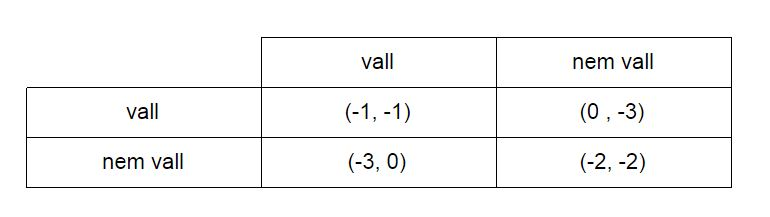
\includegraphics[width=\linewidth]{images/prisoners}
	\captionof{figure}{Fogolydilemma: két elkülönített fogoly dönthet, hogy hallgat vagy vall a másik ellen. A mátrix a nyereségeket (börtönben töltött évek) szemlélteti\label{fig:prisoners}}
\end{figure}
\end{frame}


\subsection{Játékelmélet a biológiában}
\begin{frame}
\frametitle{Játékelmélet a biológiában}
\begin{itemize}
	\item evolúciós játékok
	\item fitnesz mint nyereség
	\item evolúciósan stabil stratégia
\end{itemize}
\end{frame}
